\documentclass[11pt]{article}
\usepackage[a4paper,margin=1in]{geometry}
\usepackage{amsmath,amssymb,amsthm}
\usepackage{graphicx}
\usepackage{booktabs}
\usepackage{hyperref}
\usepackage{float}
\usepackage{xcolor}
\usepackage{enumitem}
\hypersetup{colorlinks=true,linkcolor=blue,citecolor=blue,urlcolor=blue}

\newtheorem{theorem}{Theorem}
\newtheorem{proposition}{Proposition}
\newtheorem{lemma}{Lemma}
\newtheorem{corollary}{Corollary}
\newtheorem{definition}{Definition}

\title{Boundary Compensation Origin V:\
\Large Simplicial $Z_2$ Shadow-Gauge Ensembles\
\large Spectral Wilson Weights, Structural Inhomogeneous-Bond Couplings, and Finite-Graph Confinement Diagnostics}
\author{A. A. Malachevsky\\
Independent researcher\\
Boundary Compensation Origin Program (BC-Origin / BC-O)}
\date{Version v0.1.3 review manuscript, June 2026}

\begin{document}
\maketitle

\begin{abstract}
This review manuscript, updated after the statistical-bridge review, develops the next structural layer of the BC-Origin programme after the construction of non-factorizable edge holonomy in BC-Origin III and lifted phase-flow shadow kinematics in BC-Origin IV. The central question is whether the holonomy data of multi-shadow geometry can generate gauge-type cycle weights without inserting a Wilson action by hand.

Let $\mathcal K=(V,E,F_2)$ be a finite hidden-index two-dimensional simplicial complex, let $K_{ij}=K(n_i,n_j)\ge 0$ be a structural kernel on edges, and let $\varepsilon_{ij}\in\{-1,+1\}$ be a non-factorizable $Z_2$ edge holonomy. We define the off-diagonal holonomy-weighted structural adjacency operator
\[
(A_\varepsilon)_{ii}=0,\qquad (A_\varepsilon)_{ij}=\varepsilon_{ij}K_{ij}.
\]
The first main result is the closed-walk trace identity
\[
\operatorname{Tr}(A_\varepsilon^m)=\sum_{C:\ |C|=m}\Omega_C K_C,
\]
where the sum runs over closed walks of length $m$, $\Omega_C$ is the product of edge holonomies along the walk, and $K_C$ is the product of structural kernels along the same walk. In particular, for triangular cycles,
\[
\operatorname{Tr}(A_\varepsilon^3)=6\sum_{\triangle}\Omega_\triangle K_{ij}K_{jk}K_{ki}.
\]
Thus Wilson-type $Z_2$ cycle products are not externally imposed; they occur as gauge-invariant spectral trace terms of the multi-shadow holonomy operator.

The second main step is a statistical bridge. Version v0.1.3 implements the full statistical-bridge patch requested in review: the trace is not identified with an action. Instead, a finite simplicial gauge-weight ensemble is defined by
\[
Z_3(\gamma)=\sum_{\varepsilon}\exp\left(\gamma_3\operatorname{Tr}(A_\varepsilon^3)\right),
\]
or by multi-trace extensions. This converts spectral cycle observables into Wilson-like statistical weights while keeping the structural dependence in the kernel products $K_C$. The resulting ensemble is finite-dimensional, simplicial-complex-based, and toy-model-level. It is not claimed to be physical lattice quantum field theory, QCD, a continuum gauge theory, or an empirical confinement model. Its controlled contribution is narrower but nontrivial: it shows how $Z_2$ gauge-cycle weights and inhomogeneous structural couplings arise from BC-Origin spectral geometry.
\end{abstract}

\paragraph{Revision note for v0.1.3.}
This review manuscript implements the full reviewer statistical-bridge patch. The spectral trace is explicitly treated as a gauge-invariant observable / trace functional of one fixed holonomy configuration, not as an action by itself. The pure gauge-cycle derivation uses the off-diagonal holonomy adjacency operator $A_\varepsilon$, not the full shadow operator $D_\varepsilon=\Delta+\eta_DA_\varepsilon$, because the diagonal closure denominators in $D_\varepsilon$ generate additional non-cycle contributions. The ensemble appears only after summing over edge-holonomy configurations:
\[
Z_3(\gamma)=\sum_\varepsilon \exp\left(\gamma\operatorname{Tr}(A_\varepsilon^3)\right).
\]
Using the triangle trace identity, this becomes a finite simplicial $Z_2$ shadow-gauge ensemble with structurally inhomogeneous Wilson-like couplings
\[
\beta_\triangle=6\gamma K_{ij}K_{jk}K_{ki}.
\]
The revision also adds a strong-coupling/high-temperature form, simplicial two-cell terminology, deterministic inhomogeneous-bond terminology, finite-graph area-law diagnostics, and shadow-admissibility statistics. The non-claim boundary is preserved: no physical lattice QFT, QCD, continuum confinement theorem, or empirical gauge dynamics is asserted.


\tableofcontents

\section{Introduction: from trace cycles to simplicial shadow-gauge ensembles}

BC-Origin I introduced hidden oriented winding shadows and structural scale selection. BC-Origin II replaced free pairwise couplings by structural kernels $K(n_i,n_j)$. BC-Origin III introduced non-factorizable edge holonomy and genuine cycle frustration. BC-Origin IV introduced lifted phase flow and horizon events.

BC-Origin V asks a new question:
\[
\text{edge holonomy}+\text{structural kernels}\quad\Longrightarrow\quad\text{spectral trace cycle weights?}
\]
The answer is affirmative in a finite-dimensional and graph-theoretic sense. The closed spectral traces of the holonomy-weighted adjacency operator generate Wilson-cycle products automatically.

The key methodological distinction of the paper is
\[
\operatorname{Tr}(A_\varepsilon^m)\neq\text{Wilson action by itself}.
\]
Instead, $\operatorname{Tr}(A_\varepsilon^m)$ is a gauge-invariant trace functional that can be used to define a finite simplicial ensemble over holonomy configurations. This keeps the programme away from the category error of equating an observable of one fixed configuration with an action governing a statistical or path-integral sum over configurations.

\paragraph{Guiding chain.}
The controlled chain developed here is
\[
\text{holonomy}\rightarrow\text{spectral trace cycles}\rightarrow
\text{finite simplicial gauge-weight ensemble}\rightarrow
\text{Wilson-loop diagnostics}\rightarrow
\text{shadow admissibility statistics}.
\]
This is intentionally stronger than a sterile note about traces. It is a finite-dimensional spectral-gauge construction with an actual ensemble, Wilson-like cycle weights, loop observables and horizon-admissibility statistics. It is nevertheless narrower than a physical derivation of lattice quantum field theory.

\section{Hidden-index simplicial complex and structural kernels}

Let $\mathcal K=(V,E,F_2)$ be a finite two-dimensional simplicial complex whose vertices label hidden winding generators
\[
h_i=(q_i,n_i),\qquad n_i\in\mathbb Z\setminus\{0\}.
\]
A structural kernel is assigned to edges, and the declared triangular faces $F_2$ are the elementary two-cells used for Wilson-type factors:
\[
K_{ij}=K(n_i,n_j),\qquad K_{ij}=K_{ji}\ge 0.
\]
Typical examples include the Lorentzian index-space kernel
\[
K_{ij}=\frac{\eta}{1+(n_i-n_j)^2}
\]
and exponential or finite-range kernels. The normalization $\eta$ is global; it is not a pairwise fitted coupling.

\begin{definition}[Hidden-index structural two-complex]
A hidden-index structural two-complex is a tuple
\[
\mathcal K=(V,E,F_2,n,K),
\]
where $V$ is a finite vertex set, $E$ is a finite unoriented edge set, $F_2$ is a declared set of filled triangular two-cells, $n:V\to\mathbb Z\setminus\{0\}$ assigns hidden winding labels, and $K:E\to\mathbb R_{\ge 0}$ assigns symmetric structural kernel values.

A triangle $\triangle=(ijk)$ contributes as an elementary Wilson-type face only when $\triangle\in F_2$. A graph-theoretic three-cycle not declared as an element of $F_2$ is merely a closed walk and is not automatically treated as a plaquette-like two-cell.
\end{definition}

\section{$Z_2$ edge holonomy and vertex gauge equivalence}

Assign edge variables
\[
\varepsilon_{ij}\in\{-1,+1\},\qquad \varepsilon_{ij}=\varepsilon_{ji}.
\]
A vertex gauge transformation is
\[
\varepsilon_{ij}\mapsto g_i\varepsilon_{ij}g_j,\qquad g_i\in\{-1,+1\}.
\]
For a closed cycle $C=(i_0i_1\cdots i_m=i_0)$, define
\[
\Omega_C=\prod_{\ell=0}^{m-1}\varepsilon_{i_\ell i_{\ell+1}}.
\]
Then $\Omega_C$ is invariant under vertex gauge transformations.

\begin{proposition}[Cycle holonomy gauge invariance]
For any closed cycle $C$, the cycle product $\Omega_C$ is unchanged by vertex gauge transformations $\varepsilon_{ij}\mapsto g_i\varepsilon_{ij}g_j$.
\end{proposition}

\begin{proof}
Each vertex sign $g_i$ appears exactly twice in the product around a closed cycle. Since $g_i^2=1$, all vertex factors cancel.
\end{proof}

This recalls the BC-Origin III distinction:
\[
\text{vertex-factorizable signs}\neq\text{non-factorizable edge holonomy}.
\]
Only the latter can support genuine cycle-level frustration.

\section{Holonomy-weighted structural adjacency operator}

Define
\[
(A_\varepsilon)_{ii}=0,
\]
\[
(A_\varepsilon)_{ij}=\varepsilon_{ij}K_{ij}\quad\text{for }(ij)\in E,
\]
and
\[
(A_\varepsilon)_{ij}=0\quad\text{when }(ij)\notin E.
\]
The full shadow operator may later be written as
\[
D_\varepsilon(\lambda)=\Delta(\lambda)+\eta_D A_\varepsilon,
\]
where $\Delta(\lambda)=\operatorname{diag}(d_i(\lambda))$ contains closure denominators. The pure gauge-cycle trace identities are cleanest for $A_\varepsilon$, because diagonal terms in $D_\varepsilon$ produce additional non-cycle contributions.

\begin{proposition}[Gauge covariance of $A_\varepsilon$]
Let $G_g=\operatorname{diag}(g_i)$ and let $\varepsilon^g_{ij}=g_i\varepsilon_{ij}g_j$. Then
\[
A_{\varepsilon^g}=G_g A_\varepsilon G_g.
\]
Consequently, $A_\varepsilon$ and $A_{\varepsilon^g}$ have the same spectrum and the same trace powers.
\end{proposition}

\begin{proof}
The $(i,j)$ entry of $G_g A_\varepsilon G_g$ is $g_i\varepsilon_{ij}K_{ij}g_j$, which equals $(A_{\varepsilon^g})_{ij}$. Similarity by $G_g=G_g^{-1}$ preserves the spectrum and trace powers.
\end{proof}

\begin{figure}[H]
\centering
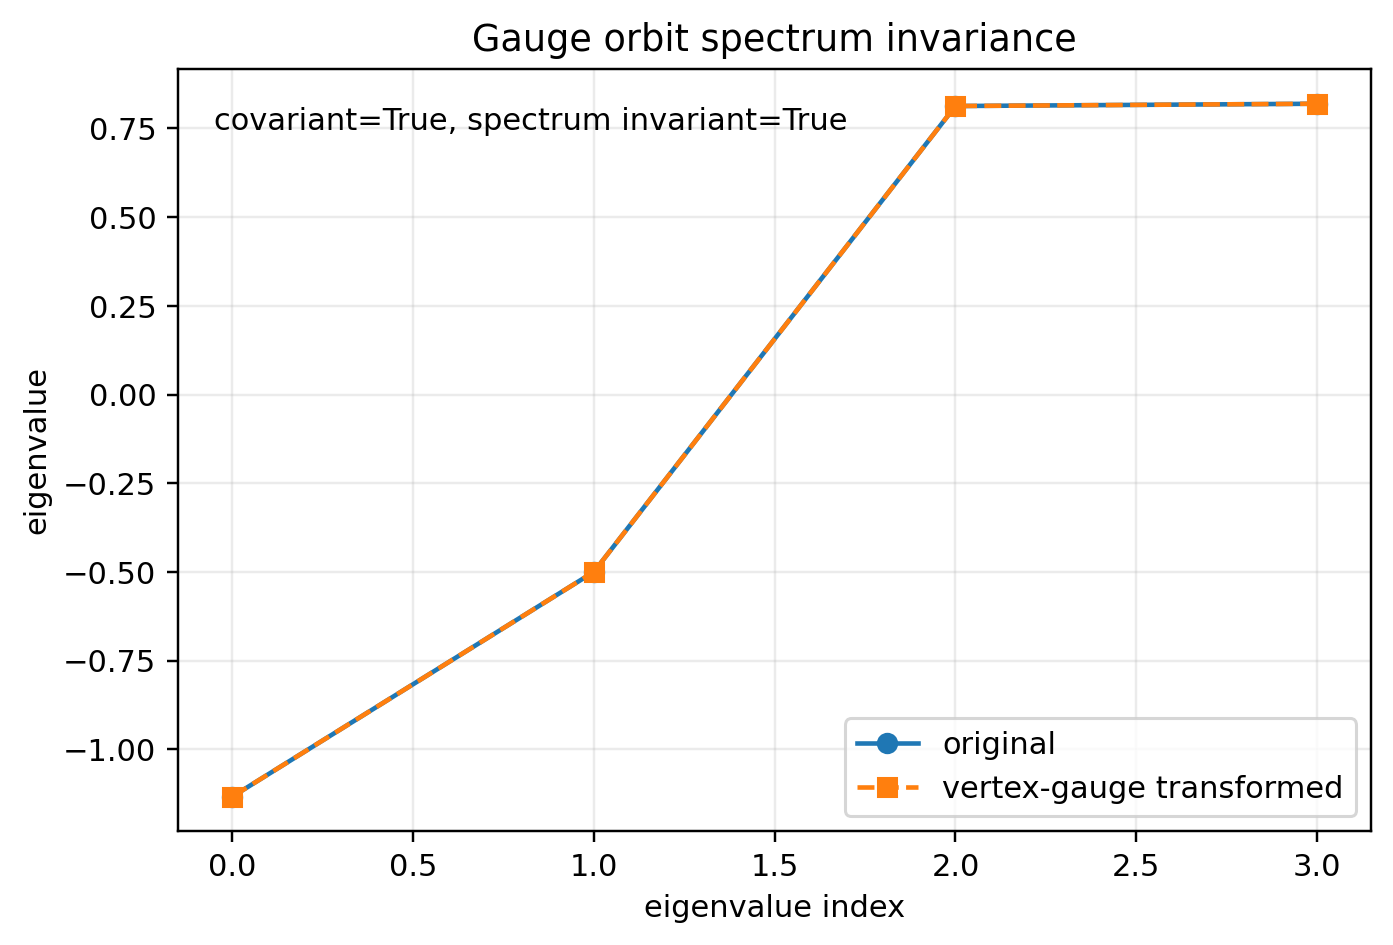
\includegraphics[width=.78\linewidth]{../origin_v/figures/gauge_orbit_spectrum_invariance.png}
\caption{Gauge orbit spectrum invariance. A vertex sign redefinition changes edge signs but preserves the spectrum of the holonomy-weighted adjacency operator.}
\end{figure}

\section{Main theorem: spectral traces generate closed holonomy walks}

\begin{theorem}[Closed-walk trace identity]
For the holonomy-weighted adjacency operator $A_\varepsilon$,
\[
\operatorname{Tr}(A_\varepsilon^m)=
\sum_{i_0,\dots,i_{m-1}}
(A_\varepsilon)_{i_0i_1}(A_\varepsilon)_{i_1i_2}\cdots(A_\varepsilon)_{i_{m-1}i_0}.
\]
Equivalently,
\[
\operatorname{Tr}(A_\varepsilon^m)=\sum_{C:\ |C|=m}\Omega_CK_C,
\]
where the sum runs over closed walks of length $m$,
\[
\Omega_C=\prod_{(ij)\in C}\varepsilon_{ij},
\]
and
\[
K_C=\prod_{(ij)\in C}K_{ij}.
\]
Thus every closed-walk term in the spectral trace carries a gauge-invariant holonomy factor.
\end{theorem}

\begin{proof}
Expand the diagonal entries of $A_\varepsilon^m$ and sum over the starting vertex. Each monomial corresponds to a closed walk. Since each off-diagonal matrix entry factorizes as $\varepsilon_{ij}K_{ij}$, the monomial factorizes into the corresponding holonomy product $\Omega_C$ and kernel product $K_C$.
\end{proof}

This theorem is the first central result of BC-Origin V. It shows that Wilson-type cycle products are not decorative analogies; they are spectral trace coefficients of the BC-Origin holonomy-weighted structural adjacency operator.

\section{Triangle Wilson-cycle corollary}

For $m=3$, only triangular closed walks contribute on a simple graph.

\begin{corollary}[Triangle trace formula]
For a simple graph,
\[
\operatorname{Tr}(A_\varepsilon^3)=
6\sum_{i<j<k}\varepsilon_{ij}\varepsilon_{jk}\varepsilon_{ki}K_{ij}K_{jk}K_{ki}.
\]
Equivalently,
\[
\operatorname{Tr}(A_\varepsilon^3)=6\sum_{\triangle}\Omega_\triangle K_\triangle.
\]
The factor $6$ counts the two orientations and three cyclic starting points of each triangle.
\end{corollary}

\begin{figure}[H]
\centering
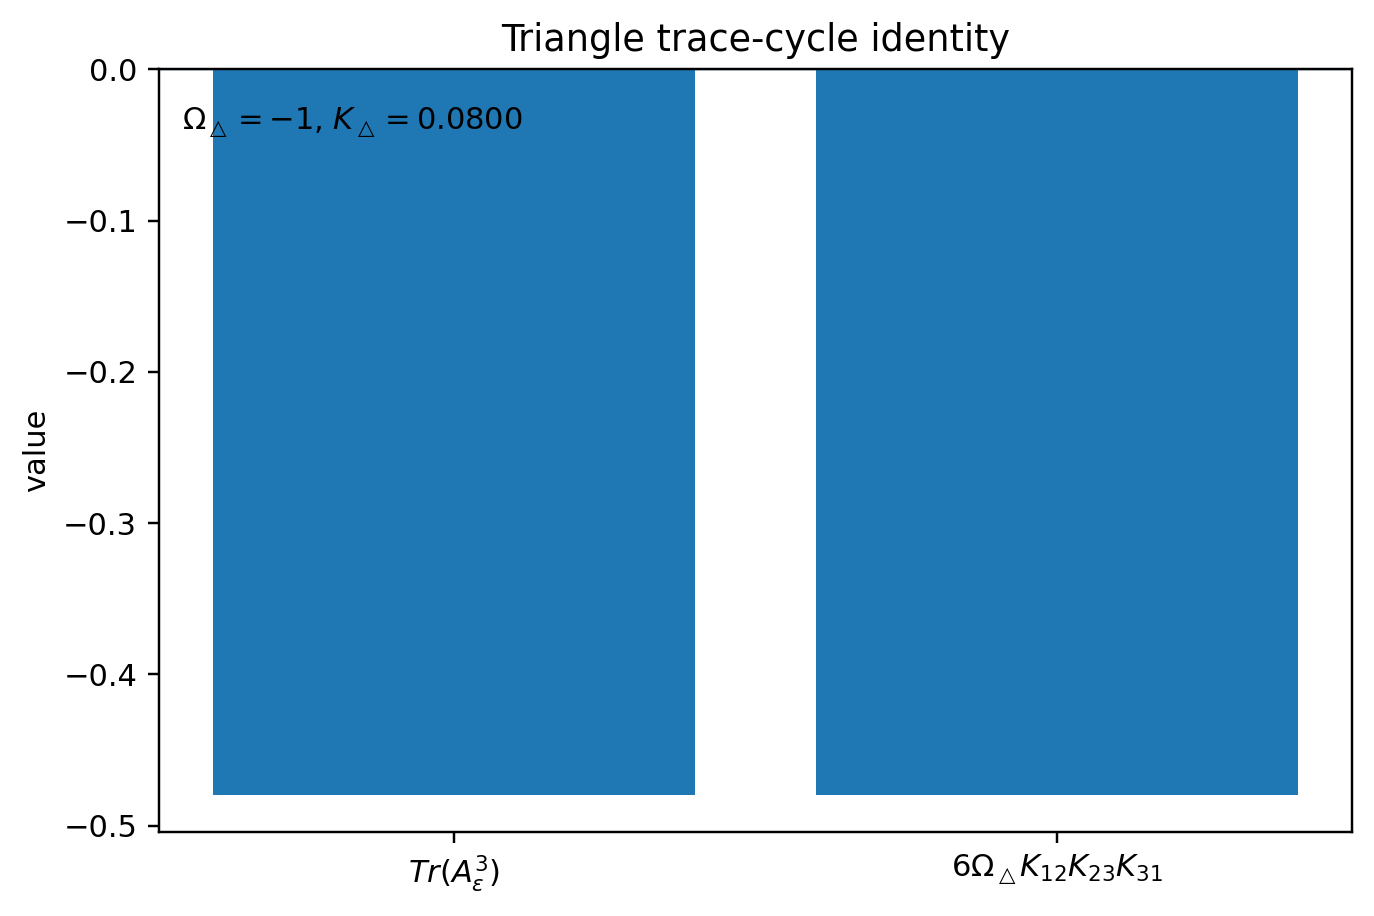
\includegraphics[width=.76\linewidth]{../origin_v/figures/trace_cycle_triangle_identity.png}
\caption{Triangle trace-cycle identity. The direct spectral trace $\operatorname{Tr}(A_\varepsilon^3)$ agrees with the Wilson-cycle expression $6\Omega_\triangle K_{12}K_{23}K_{31}$.}
\end{figure}

This is the minimal BC-Origin Wilson-cycle emergence statement.


\section{The statistical bridge: from spectral trace observables to a finite $Z_2$ gauge-weight ensemble}

BC-Origin III introduced non-factorizable edge holonomies
\[
\varepsilon_{ij}\in\{-1,+1\}
\]
on a finite hidden-index graph. Under a vertex gauge transformation
\[
\varepsilon_{ij}\mapsto g_i\varepsilon_{ij}g_j,\qquad g_i\in\{-1,+1\},
\]
cycle products
\[
\Omega_C=\prod_{(ij)\in C}\varepsilon_{ij}
\]
are gauge-invariant. BC-Origin V asks whether these gauge-invariant cycle products are merely imposed by hand, or whether they arise naturally from spectral invariants of the shadow operator.

To isolate the pure gauge-cycle part, define the off-diagonal holonomy-weighted structural adjacency operator
\[
(A_\varepsilon)_{ii}=0,
\]
\[
(A_\varepsilon)_{ij}=\varepsilon_{ij}K_{ij}\quad\text{for }(ij)\in E,
\]
where $K_{ij}=K(n_i,n_j)\ge0$ is the structural kernel inherited from the hidden winding-index geometry.

The full shadow operator used for admissibility diagnostics will later be written as
\[
D_\varepsilon=\Delta+\eta_D A_\varepsilon,
\]
where
\[
\Delta=\operatorname{diag}(d_1,\ldots,d_N)
\]
contains closure denominators. However, the clean Wilson-cycle trace identity belongs to $A_\varepsilon$, not to $D_\varepsilon$, because diagonal closure terms generate additional non-cycle contributions.

For the cubic trace,
\[
\operatorname{Tr}(A_\varepsilon^3)=\sum_{i,j,k}(A_\varepsilon)_{ij}(A_\varepsilon)_{jk}(A_\varepsilon)_{ki}.
\]
Substituting the structural edge form gives
\[
(A_\varepsilon)_{ij}(A_\varepsilon)_{jk}(A_\varepsilon)_{ki}
=(\varepsilon_{ij}K_{ij})(\varepsilon_{jk}K_{jk})(\varepsilon_{ki}K_{ki}).
\]
Thus
\[
(A_\varepsilon)_{ij}(A_\varepsilon)_{jk}(A_\varepsilon)_{ki}
=\Omega_{ijk}\,K_{ij}K_{jk}K_{ki},
\]
where
\[
\Omega_{ijk}=\varepsilon_{ij}\varepsilon_{jk}\varepsilon_{ki}
\]
is the $Z_2$ Wilson cycle around the triangle $(ijk)$. Therefore, on a simple undirected triangular graph,
\[
\operatorname{Tr}(A_\varepsilon^3)=6\sum_{\triangle}\Omega_\triangle K_\triangle,
\]
with
\[
K_\triangle=K_{ij}K_{jk}K_{ki}.
\]
The factor $6$ counts the two orientations and the three cyclic starting points of each triangle.

This establishes the first bridge:
\[
\text{spectral trace cycle}\quad\Longrightarrow\quad
\text{$Z_2$ Wilson-cycle term with structural kernel weight}.
\]

However, this trace is not yet an action. It is a gauge-invariant observable of one fixed holonomy configuration $\varepsilon$. A statistical or path-sum model appears only after summing over all edge-holonomy configurations.

We therefore define the finite graph partition function
\[
Z_3(\gamma)=\sum_{\varepsilon\in\{-1,+1\}^{E}}
\exp\left(\gamma\operatorname{Tr}(A_\varepsilon^3)\right).
\]
Using the trace identity,
\[
Z_3(\gamma)=\sum_{\varepsilon}\exp\left(6\gamma\sum_{\triangle}\Omega_\triangle K_\triangle\right).
\]
Equivalently,
\[
Z_3(\gamma)=\sum_{\varepsilon}\exp\left(\sum_{\triangle}\beta_\triangle\Omega_\triangle\right),
\]
where the effective triangular Wilson weight is
\[
\beta_\triangle=6\gamma K_{ij}K_{jk}K_{ki}.
\]
Thus the Wilson-like action is not inserted as a primitive postulate. It is generated by using the spectral trace functional of the holonomy-weighted structural adjacency operator as the energy functional of a finite $Z_2$ gauge-weight ensemble.

The global parameter $\gamma$ is an ensemble-control parameter. It controls how strongly the statistical sum weights the cubic spectral trace of the holonomy adjacency operator. It is analogous to an inverse temperature or trace-weighting strength, but in BC-Origin it is not identified with physical temperature, physical time, or a fundamental gauge coupling.

The limiting readings are purely ensemble-theoretic. For $\gamma\to 0$, edge-holonomy configurations are nearly unweighted and the gauge background is maximally fluctuating. For large positive $\gamma$, configurations with larger structural trace contribution are exponentially favored, so the ensemble becomes more strongly organized by the declared face weights $K_\triangle$. The local deterministic inhomogeneous coupling structure remains determined by the structural kernel products $K_\triangle$.

\begin{definition}[BC-Origin finite simplicial $Z_2$ shadow-gauge ensemble]
Given a structural two-complex $\mathcal K=(V,E,F_2,n,K)$, define
\[
Z(\gamma)=\sum_{\varepsilon\in\{-1,+1\}^E}
\exp\left(\sum_{\triangle\in F_2}\beta_\triangle\Omega_\triangle\right),
\]
where
\[
\beta_\triangle=6\gamma K_\triangle.
\]
This is the finite simplicial $Z_2$ shadow-gauge ensemble generated by the cubic trace of $A_\varepsilon$ on the declared triangular two-cells.
\end{definition}

This definition is intentionally finite-dimensional. It is not a continuum limit and not a physical path integral over spacetime gauge fields.

\section{Strong-coupling / high-temperature form and Wilson-like local weights}

For one triangle,
\[
\exp(\beta_\triangle\Omega_\triangle)=
\cosh(\beta_\triangle)
\left[1+\Omega_\triangle\tanh(\beta_\triangle)\right],
\]
where
\[
\beta_\triangle=6\gamma K_{ij}K_{jk}K_{ki}.
\]
Thus the effective Wilson-like triangle weight is structurally modulated:
\[
u_\triangle=\tanh(6\gamma K_{ij}K_{jk}K_{ki}).
\]
Unlike a uniform Wilson lattice action, BC-Origin produces inhomogeneous structural weights because $K_{ij}$ depends on hidden winding-index geometry.

The parameter $u_\triangle$ is the natural finite-simplicial-complex strong-coupling/high-temperature expansion variable. Small $|u_\triangle|$ corresponds to a strongly fluctuating holonomy ensemble on the declared finite complex, while large $|u_\triangle|$ favors ordered triangle holonomies. In this manuscript such statements are finite-graph ensemble statements only; thermodynamic phase transitions require a graph-size limit and finite-size scaling, which are outside the claim set of v0.1.3.

\begin{figure}[H]
\centering
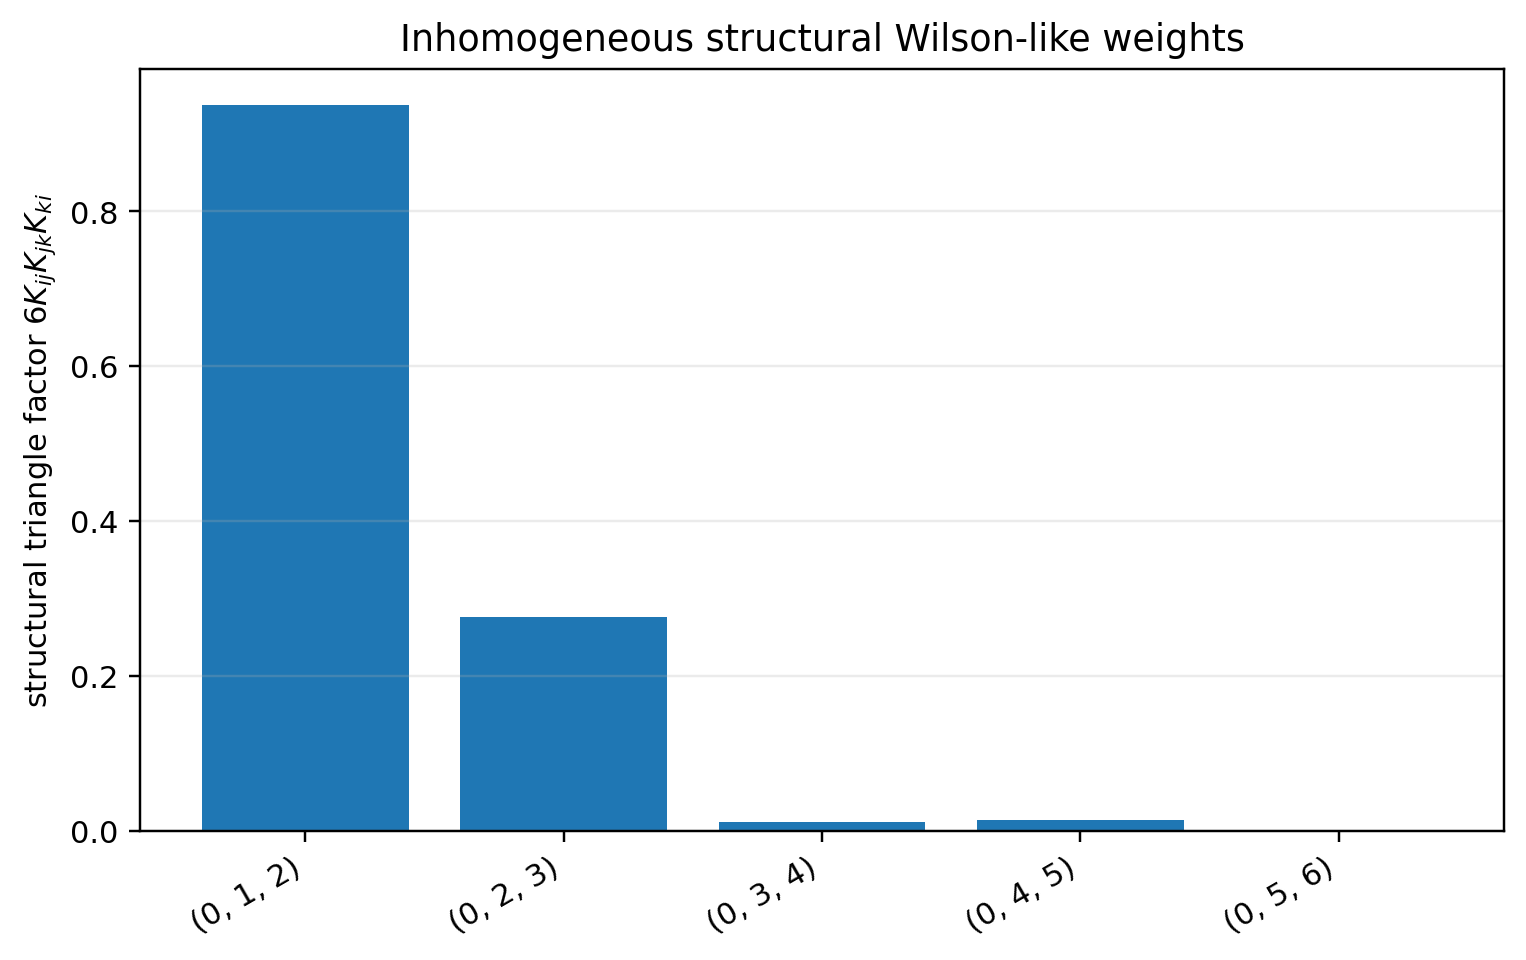
\includegraphics[width=.78\linewidth]{../origin_v/figures/deterministic_inhomogeneous_bond_weights.png}
\caption{Structural inhomogeneity. Different triangles acquire different Wilson-like weights because the kernel products $K_{ij}K_{jk}K_{ki}$ depend on hidden winding-index geometry. No stochastic disorder average is used; these weights are deterministic once the hidden labels and kernel are fixed.}
\end{figure}

\section{Finite simplicial interpretation: triangles as elementary 2-cells}

The appearance of triangular cycles is not an error. It indicates that the natural finite structure is not necessarily a hypercubic lattice, but a graph or simplicial complex whose elementary closed 2-cells may be triangles.

If a 2-complex structure is declared, triangle holonomies can be interpreted as plaquette-like variables on triangular faces. The article does not claim a continuum limit, Regge calculus, dynamical triangulations, or quantum gravity. It only identifies the finite simplicial gauge-weight structure naturally generated by spectral trace cycles.

\section{Deterministic inhomogeneous-bond structure}

Because
\[
\beta_\triangle=6\gamma K_{ij}K_{jk}K_{ki},
\]
different triangles generally have different weights. This produces a deterministic inhomogeneous-bond $Z_2$ gauge ensemble. No quenched disorder average is performed in BC-Origin V, and no probability measure over hidden labels is assumed. A stochastic disorder model would arise only after adding an explicit probability law on hidden-index data and averaging the appropriate thermodynamic quantities; that extension is outside the present manuscript.

\section{Finite-graph crossover and confinement-like diagnostics}

The ensemble supports observables analogous to standard lattice-gauge diagnostics, but only on the declared finite graph or finite simplicial complex. Define the average triangle holonomy
\[
\langle\Omega_\triangle\rangle_\gamma
=\frac{1}{|F_2|}\sum_{\triangle\in F_2}\langle\Omega_\triangle\rangle_\gamma,
\]
and a finite-graph frustration energy
\[
E_F(\gamma)=1-\langle\Omega_\triangle\rangle_\gamma.
\]
The derivative or variance of this quantity under a sweep of $\gamma$ may show a finite-size crossover or susceptibility peak. The paper does not call this a thermodynamic phase transition unless an appropriate sequence of graph refinements and scaling limit is supplied.

For closed cycles $C$ one may compute Wilson-loop-like expectations $\langle\Omega_C\rangle_\gamma$ and compare $-\log|\langle\Omega_C\rangle_\gamma|$ with a declared enclosed triangle count. This is a finite-graph area-law diagnostic, not a proof of continuum confinement.

\section{Coupling to shadow denominators}

The observable shadow operator may be written
\[
D_\varepsilon(\lambda)=\Delta(\lambda)+\eta_D A_\varepsilon,
\]
where
\[
\Delta(\lambda)=\operatorname{diag}(d_i(\lambda)).
\]
The eigen-denominators $\lambda_a(D_\varepsilon)$ define local admissibility through
\[
\lambda_{\min}(D_\varepsilon)>0.
\]
In the ensemble, one may define an admissibility fraction
\[
P_{\rm adm}(\gamma)=
\left\langle \mathbf 1_{\lambda_{\min}(D_\varepsilon)>0}\right\rangle_\gamma.
\]
This gives a finite graph diagnostic of how holonomy ensembles affect shadow localization. No particle mass, physical confinement, or empirical matter field is claimed.

\begin{figure}[H]
\centering
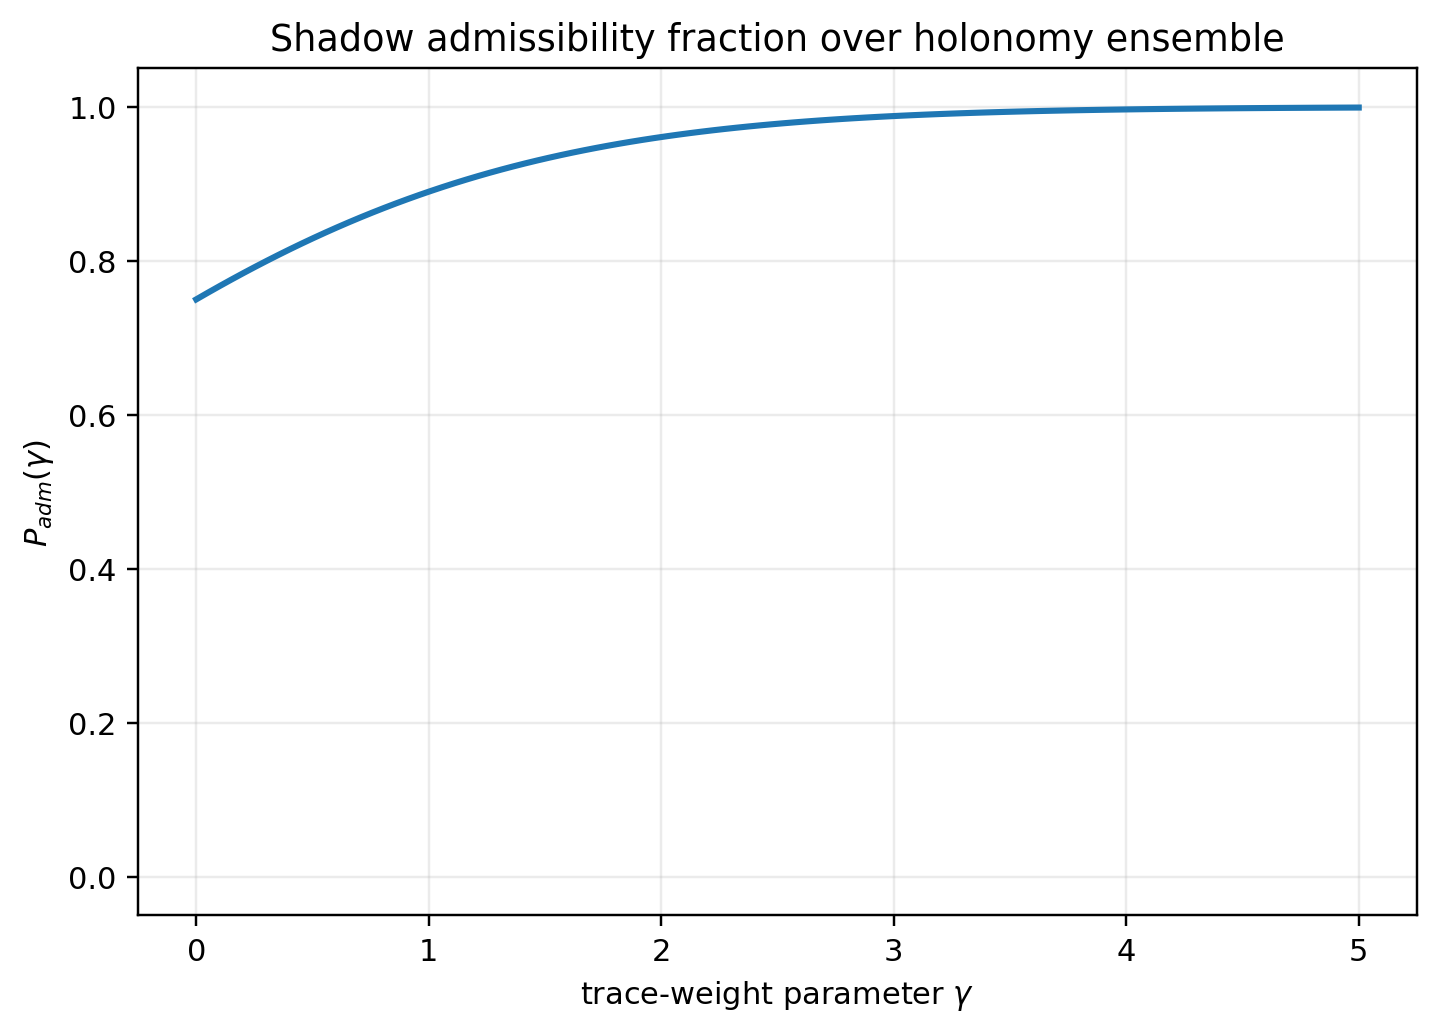
\includegraphics[width=.78\linewidth]{../origin_v/figures/shadow_admissibility_fraction.png}
\caption{Shadow admissibility fraction over a finite holonomy ensemble. This is a finite graph diagnostic of local shadow admissibility, not a physical matter-confinement theorem.}
\end{figure}

\section{Wilson-loop diagnostics and confinement analogues}

For a closed cycle $C$, define the ensemble expectation
\[
\langle \Omega_C\rangle_\gamma=
\frac{1}{Z}\sum_\varepsilon \Omega_C
\exp\left(\gamma_3\operatorname{Tr}(A_\varepsilon^3)\right).
\]
On finite graphs, one can measure whether larger cycles show rapid decay with a chosen notion of enclosed area. This is only a finite graph area-law diagnostic, not a proof of continuum confinement.

Allowed statement:
\[
\text{The ensemble supports finite-graph Wilson-loop diagnostics.}
\]
Forbidden statement:
\[
\text{BC-Origin proves physical confinement.}
\]

\begin{figure}[H]
\centering
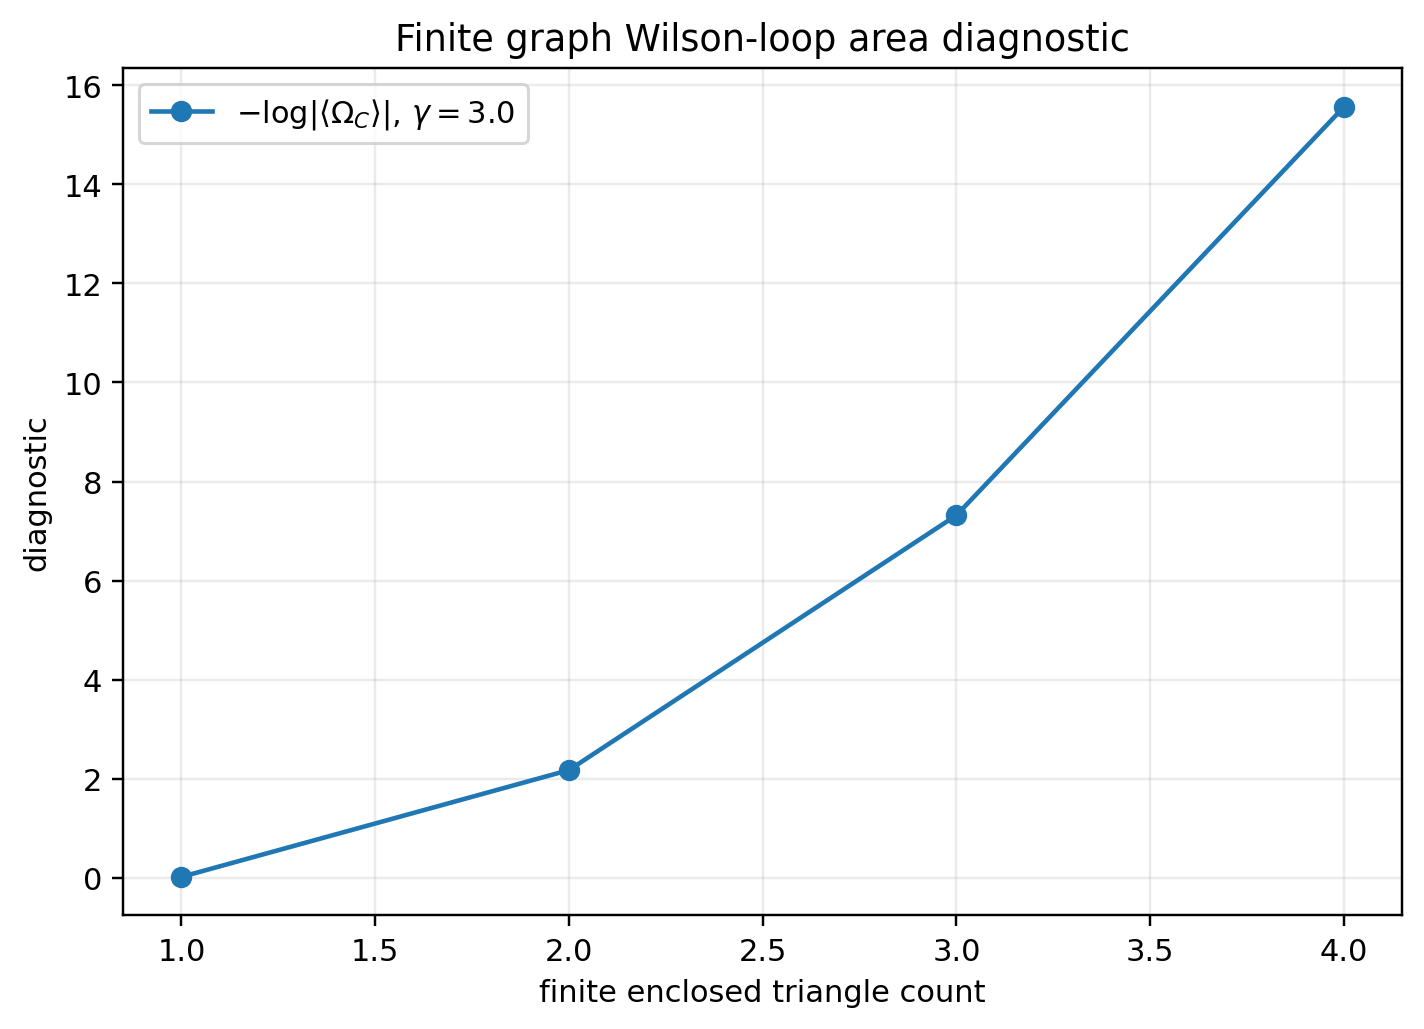
\includegraphics[width=.78\linewidth]{../origin_v/figures/finite_graph_area_law_diagnostic.png}
\caption{Finite graph area-law diagnostic. The figure shows how Wilson-loop diagnostics can be computed on a finite triangulated fan. No continuum confinement theorem is claimed.}
\end{figure}

\section{Minimal exact examples}

\subsection{Single triangle}

For three vertices and three edges,
\[
\operatorname{Tr}(A_\varepsilon^3)=6\Omega_\triangle K_{12}K_{23}K_{31}.
\]
The partition function is
\[
Z=8\cosh(6\gamma K_\triangle),
\]
if summing over all edge sign configurations. The expectation is
\[
\langle\Omega_\triangle\rangle=\tanh(6\gamma K_\triangle).
\]

\begin{figure}[H]
\centering
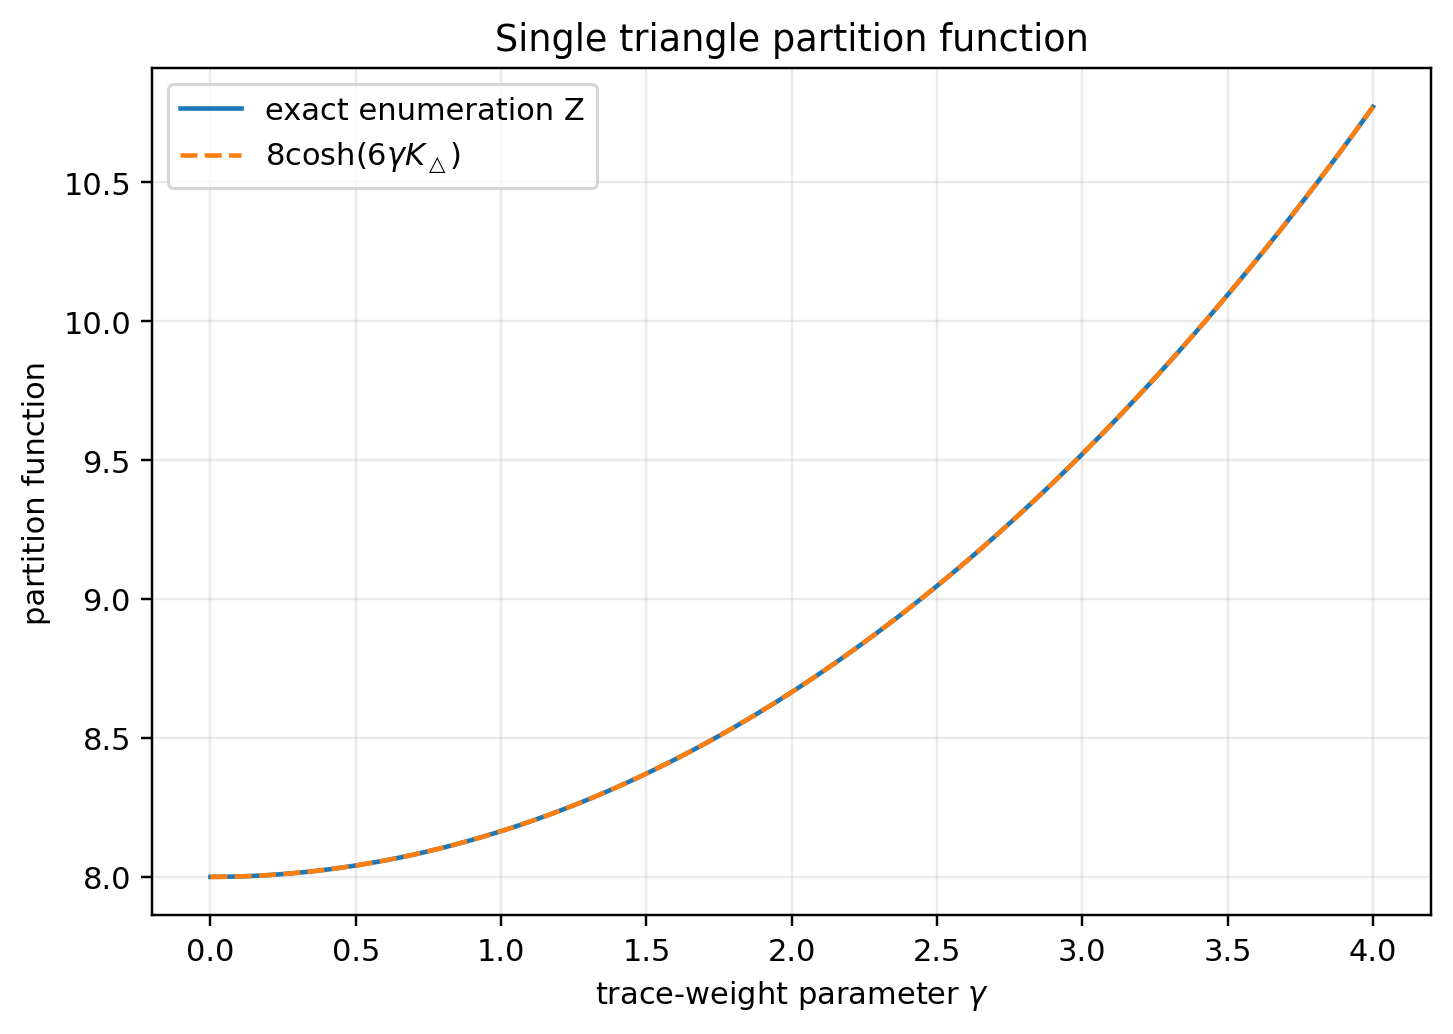
\includegraphics[width=.78\linewidth]{../origin_v/figures/single_triangle_exact_partition.png}
\caption{Single triangle partition function. Exact enumeration agrees with the analytic expression $8\cosh(6\gamma K_\triangle)$.}
\end{figure}

\begin{figure}[H]
\centering
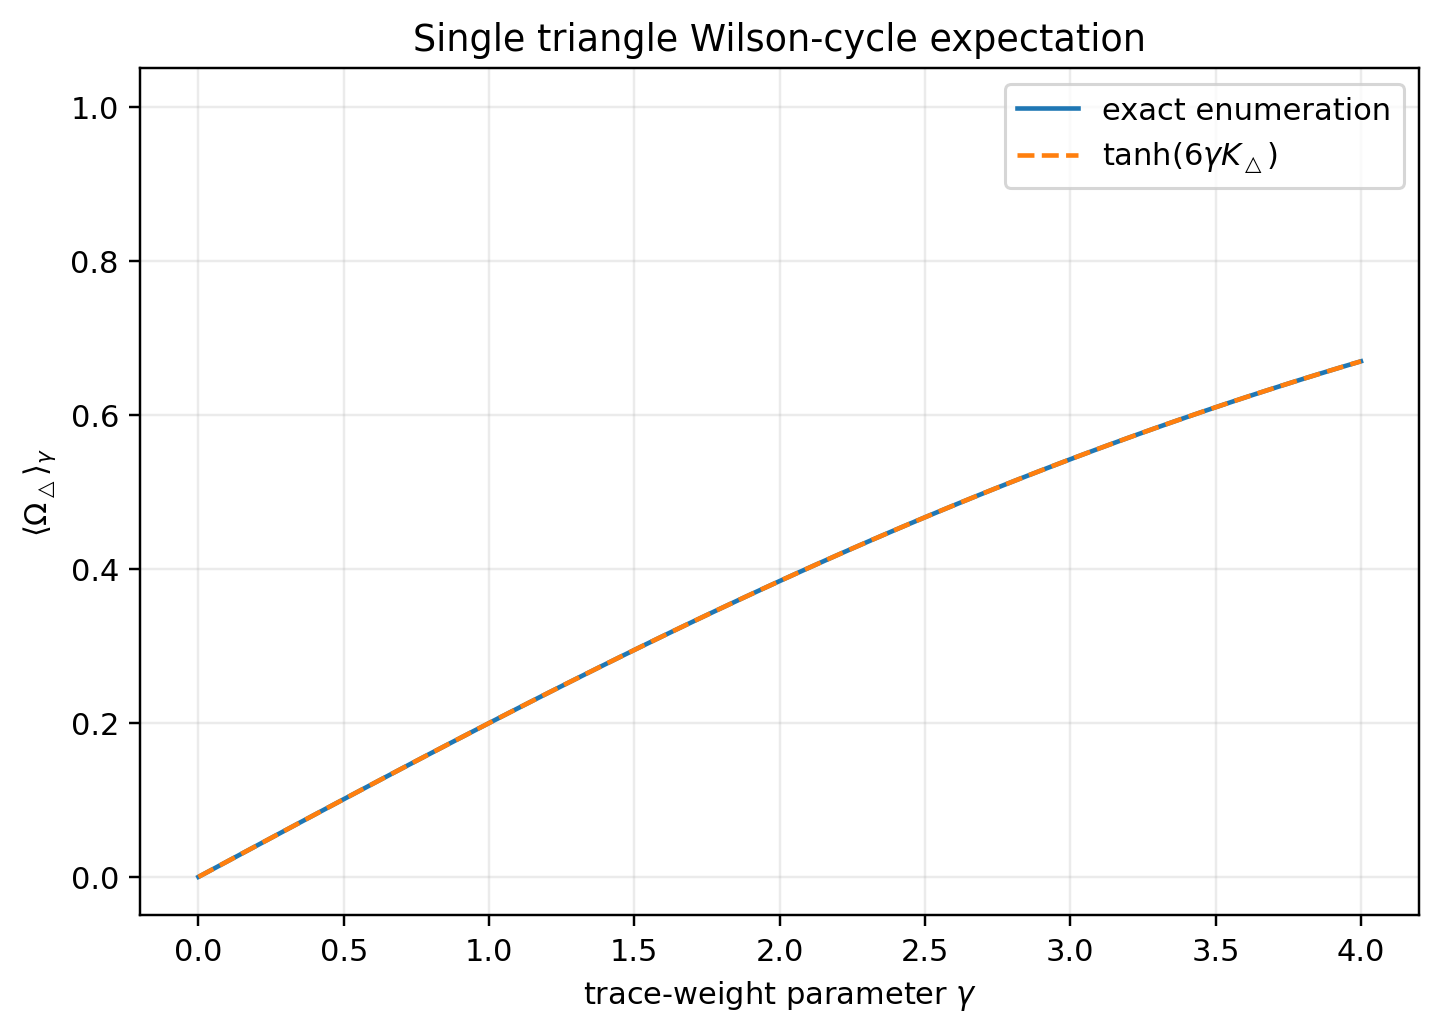
\includegraphics[width=.78\linewidth]{../origin_v/figures/single_triangle_wilson_expectation.png}
\caption{Single triangle Wilson-cycle expectation. Exact enumeration agrees with $\tanh(6\gamma K_\triangle)$.}
\end{figure}

\subsection{Two triangles sharing one edge}

The ensemble contains two coupled triangle holonomies because the same edge sign participates in both cycles. This is the smallest nontrivial interacting gauge-weight example.

\begin{figure}[H]
\centering
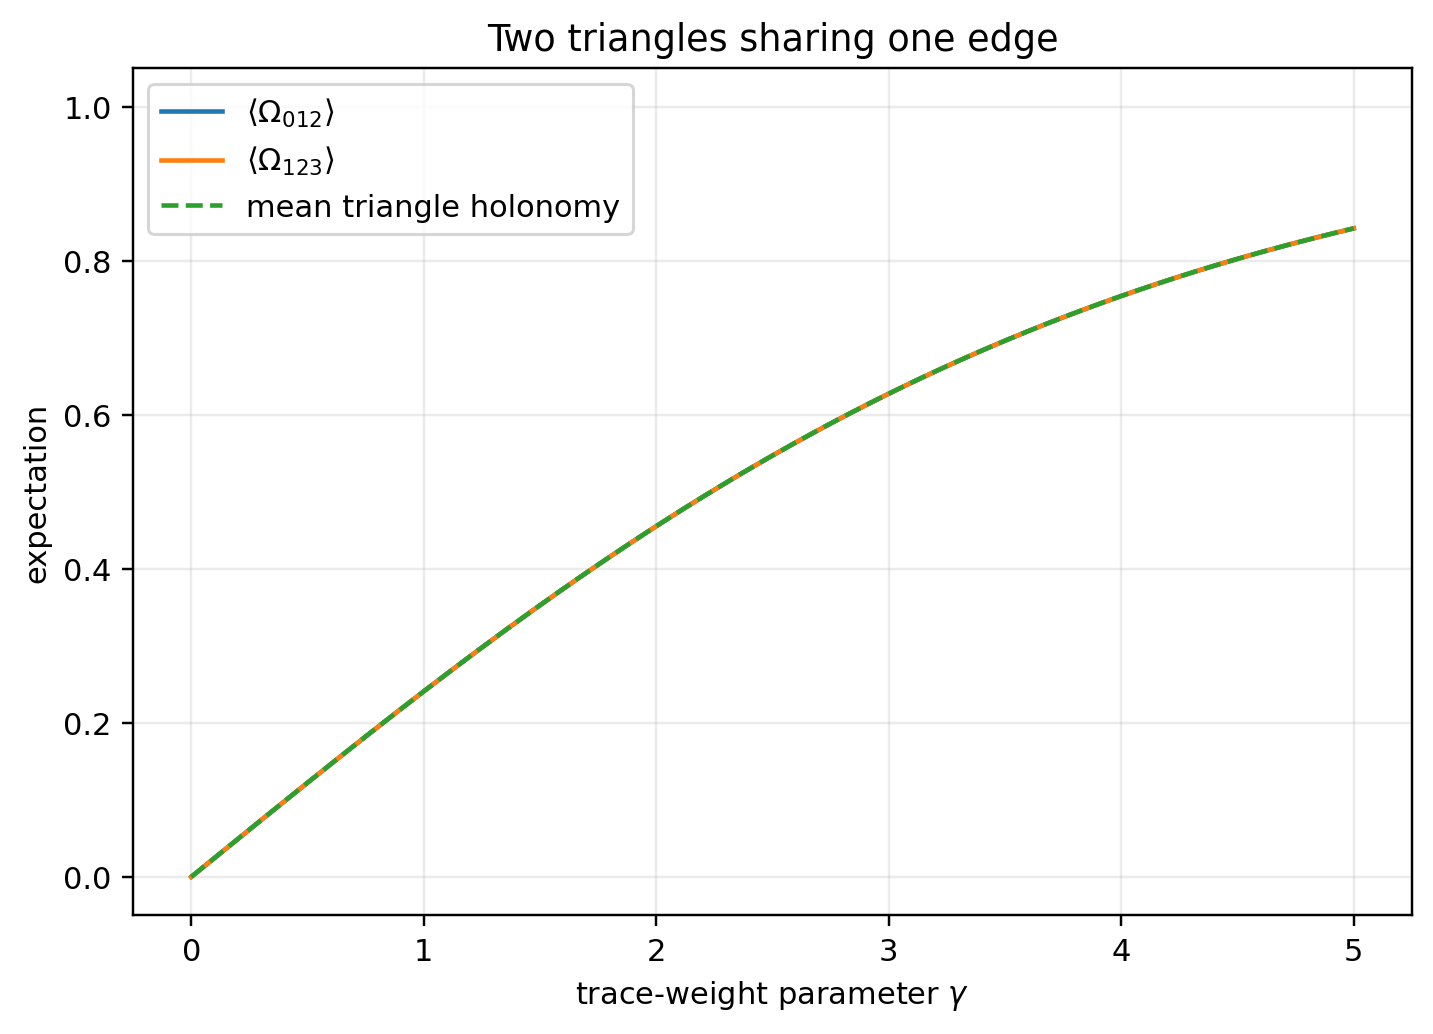
\includegraphics[width=.78\linewidth]{../origin_v/figures/two_triangle_shared_edge_expectations.png}
\caption{Two triangles sharing one edge. The finite simplicial ensemble couples triangle holonomies through shared edge signs.}
\end{figure}

\subsection{Finite-graph crossover diagnostics}

On finite graphs one should speak of crossovers, finite-size susceptibility peaks, or diagnostic changes, not thermodynamic phase transitions. A thermodynamic transition requires a size limit and finite-size scaling.

\begin{figure}[H]
\centering
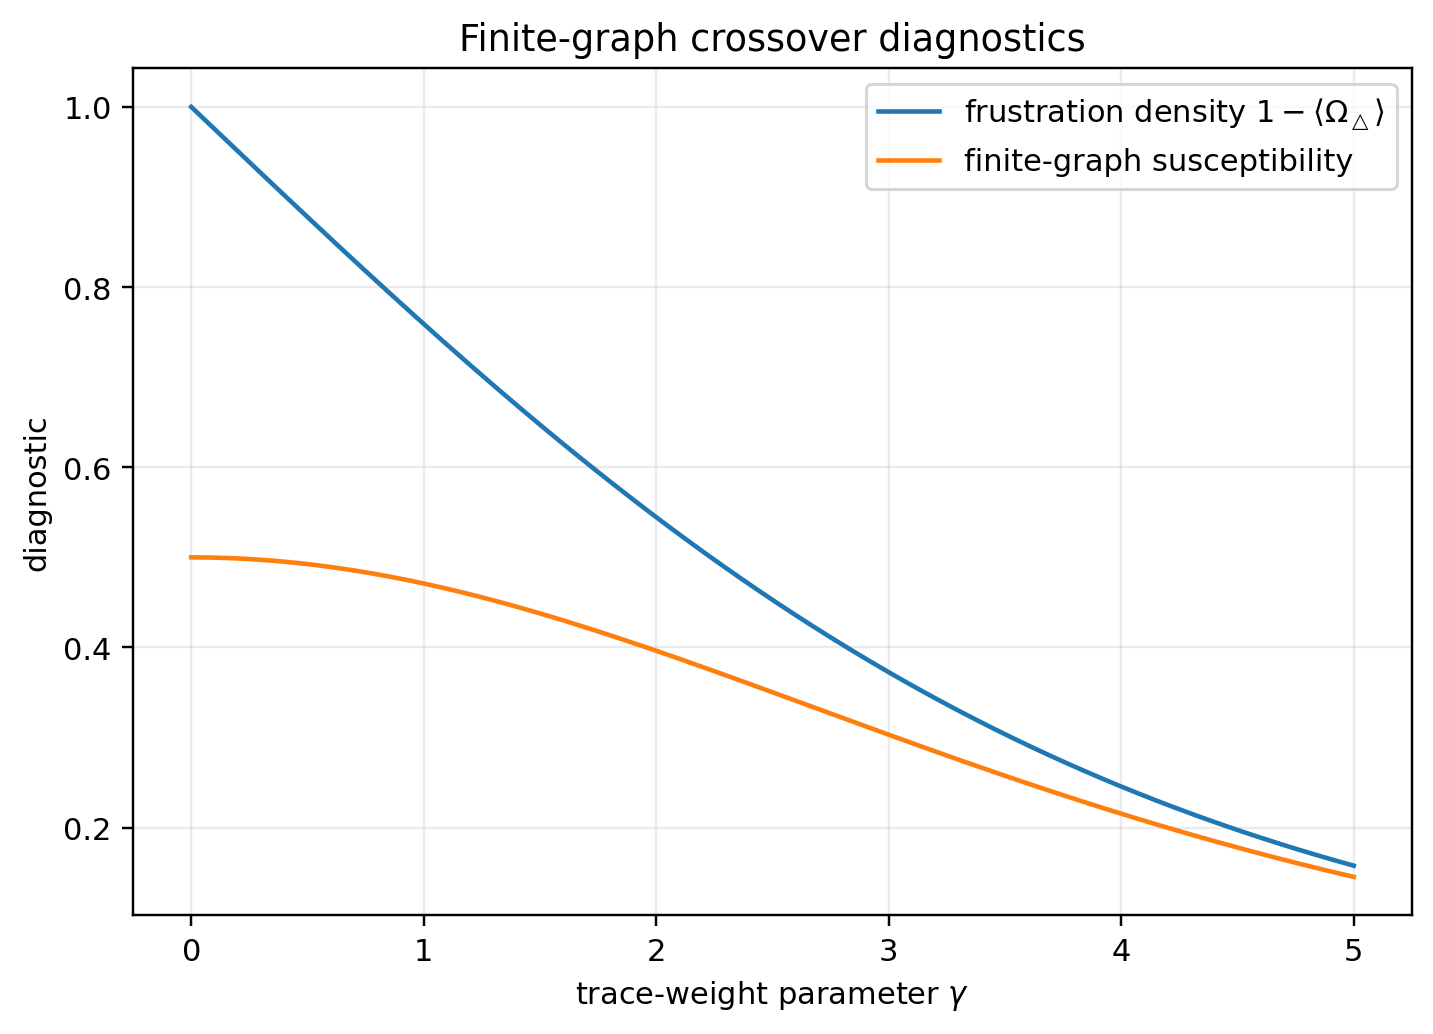
\includegraphics[width=.78\linewidth]{../origin_v/figures/plaquette_energy_and_susceptibility.png}
\caption{Finite-graph frustration and susceptibility diagnostics. These are not thermodynamic phase-transition claims.}
\end{figure}

\section{Software companion}

The software companion consists of a reproducible Python layer and an interactive HTML layer.

\paragraph{Python layer.} The Python package performs exact enumeration for small graphs, verifies trace identities, computes finite graph partition functions, measures Wilson-cycle expectations, and computes shadow-admissibility fractions. It also includes an optional Metropolis sampler for larger exploratory graphs, but exact enumeration remains primary for review examples.

\paragraph{HTML layer.} The interactive HTML lab visualizes the selected finite graph, edge holonomies, triangle products $\Omega_\triangle$, exact ensemble diagnostics, and shadow admissibility. It is a reader-facing demonstration, not a physical simulator.

\begin{figure}[H]
\centering
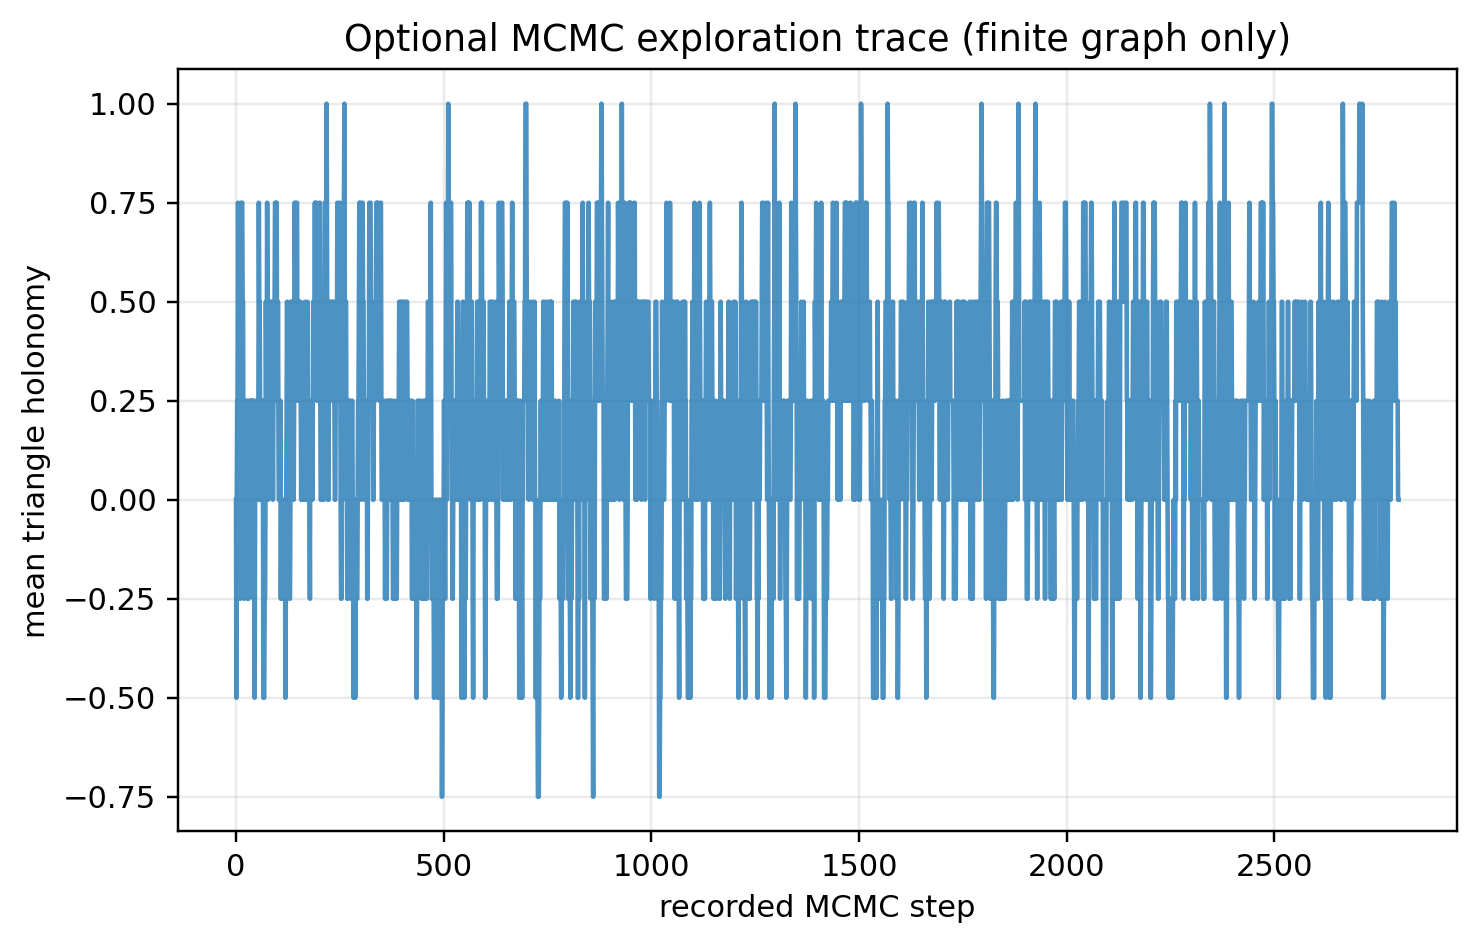
\includegraphics[width=.78\linewidth]{../origin_v/figures/mcmc_thermalization_trace.png}
\caption{Optional MCMC exploration trace on a larger finite graph. This is a finite graph sampling tool and not a physical QFT simulation.}
\end{figure}

\section{Relation to BC-Origin I--IV}

\begin{itemize}[leftmargin=2em]
\item BC-Origin I: closure-selected shadows.
\item BC-Origin II: structural kernels.
\item BC-Origin III: non-factorizable edge holonomy.
\item BC-Origin IV: lifted phase-flow and horizon events.
\item BC-Origin V: spectral traces generate gauge-cycle weights and finite simplicial ensembles.
\end{itemize}

The present article should not be read as a replacement for the earlier modules. It is a structural bridge from static holonomy to finite statistical gauge-weight ensembles.

\section{Controlled claims}

The paper claims:
\begin{enumerate}[leftmargin=2em]
\item $Z_2$ edge holonomy is naturally represented by signed structural adjacency operators.
\item Closed spectral traces generate closed-walk holonomy products.
\item Triangle Wilson-cycle terms appear in $\operatorname{Tr}(A_\varepsilon^3)$.
\item A finite simplicial gauge-weight ensemble can be defined from spectral trace functionals.
\item Structural kernels induce inhomogeneous Wilson-like cycle weights.
\item Shadow admissibility can be averaged over the finite holonomy ensemble.
\item Finite graph Wilson-loop and admissibility diagnostics provide a controlled confinement-like diagnostic language.
\end{enumerate}

\section{Non-claims and limitations}

The paper does not claim:
\begin{enumerate}[leftmargin=2em]
\item derivation of physical lattice quantum field theory;
\item derivation of QCD or Standard Model gauge theory;
\item proof of continuum confinement;
\item empirical spin-glass dynamics;
\item physical path integral over real fields;
\item derivation of matter particles;
\item quantum gravity;
\item continuum limit;
\item physical time dynamics;
\item experimental prediction.
\end{enumerate}

\section{Conclusion}

BC-Origin V shows that the non-factorizable holonomy introduced in BC-Origin III is not merely a static sign decoration. Once inserted into a structural adjacency operator, it appears automatically in spectral trace cycles. By using these trace functionals as weights in a finite simplicial ensemble, the programme obtains a controlled statistical bridge from shadow holonomy to Wilson-like gauge-cycle weights.

This is not yet physical lattice quantum field theory. It is a finite-dimensional spectral-gauge ensemble generated from BC-Origin structural data. The next natural task is to determine which finite graph confinement-like diagnostics are robust under graph refinement, kernel deformation, and admissibility threshold changes.

\appendix
\section{Formal review checklist}

Before publication, reviewers should verify:
\begin{enumerate}[leftmargin=2em]
\item equation numbering and theorem numbering;
\item trace/action distinction;
\item gauge invariance of cycle products;
\item exact single triangle formulas;
\item exact enumeration checks in the software;
\item conservative confinement-language discipline;
\item rendering of all figures and formulas.
\end{enumerate}

\section{Zenodo metadata draft}

\textbf{Title:} Boundary Compensation Origin V: Simplicial $Z_2$ Shadow-Gauge Ensembles and Spectral Wilson Weights.\\
\textbf{Version:} v0.1.3 review manuscript.\\
\textbf{Keywords:} Boundary Compensation; BC-Origin; $Z_2$ gauge ensemble; Wilson loop; spectral trace; structural kernel; finite graph; holonomy; shadow admissibility; toy model.

\end{document}
